\documentclass[journal]{IEEEtran}
\ifCLASSINFOpdf \else \fi
\usepackage{xcolor} 
\usepackage{graphicx}

% *** MATH PACKAGES ***
\usepackage[cmex10]{amsmath}
\usepackage{amssymb}

%
% *** Algorithm PACKAGES ***
\usepackage{algorithmic}
%
% *** ALIGNMENT PACKAGES ***
\usepackage{array}
%
% *** SUBFIGURE PACKAGES ***
\ifCLASSOPTIONcompsoc
 \usepackage[caption=false,font=normalsize,labelfont=sf,textfont=sf]{subfig}
\else
 \usepackage[caption=false,font=footnotesize]{subfig}
\fi
%
% *** PDF, URL AND HYPERLINK PACKAGES ***
\usepackage{url}
%
% correct bad hyphenation here
\hyphenation{op-tical net-works semi-conduc-tor}
\usepackage[noadjust]{cite}

\def\spacingset#1{\renewcommand{\baselinestretch}%
	{#1}\small\normalsize} \spacingset{1.4}




\begin{document}

\title{The Algorithmic Prediction in Insurance: Risk Prediction Model }

\author{{Georg Ben Gottwald & Xueru Ma}% <-this % stops a space

 Department of Statistical Sciences,University of Toronto
\thanks{}% <-this % stops a space
\thanks{}}

% The paper headers
\markboth{}%
{Shell \MakeLowercase{\textit{et al.}}: Bare Demo of IEEEtran.cls for Journals}




% make the title area
\maketitle

% As a general rule, do not put math, special symbols or s
% in the abstract or keywords
\begin{abstract}
When compared to other insurance companies, insurance development shows how one insurance company gets people who face similar risks to buy insurance. Indirect business growth is when an insurance company gets more customers through insurance brokers and agents. Direct business growth is when an insurance company's representatives go out and get customers directly. A customer may pay an insurance premium once or more during a specific time period, and the insurance company will gather all of the premium payments made by numerous customers. When an insured accident occurs, the insurance provider pays the agreed-upon indemnity. If the indemnity payment from the insurance company is less than the total amount of money made from insurance premiums from beginning to end, the difference is called the "underwriting profit" of the insurance company. For example, if many homeowners in different places buy insurance policies and pay insurance premiums to the insurance company, the insurance company will honor the insurance liability according to the insurance terms if the accident covered by the insurance happens. Some people might not need one at all if the insurance benefit they get when the insured event happens is much higher than the insurance premium they paid. This is because, in the case of some policyholders, the insured event might not have happened during the whole insurance period. In the insurance industry, life insurance companies can make sizable annual profits. Long-term life insurance, also referred to as savings life insurance, is distinct from general insurance in that it has different insurance income and payment options. It also has various ways to make money as a result. In some countries with developed insurance markets, life insurance companies have much lower chances of going bankrupt than general insurance companies. Collectively, insurance companies settle claims for less money than they receive in premium payments. cost and profit differences between the two types. The most important thing for insurance companies is to figure out how to make their designation systems and policies more smartly so that they can make as much money as possible. In this situation, it is very important to use more logical statistical methods to improve the big picture. Throughout the paper, we will employ academic applications of statistics, related programming languages (SQL, R), and other strategies to aid insurance companies in maximizing profits.

\par Keywords: {SQL, Insurance, Pertinent, Programming, Accordance}


\end{abstract}

% \begin{IEEEkeywords}
% IEEEtran, journal, \LaTeX, paper, template.
% \end{IEEEkeywords}

\IEEEpeerreviewmaketitle

\section{Introduction}
When choosing a policy, the insurance company's financial health and soundness may be important. Most of the time, people pay insurance premiums to cover losses that will happen over a long period of time. Because of this, it is crucial that insurance companies remain viable. In the past few years, a lot of insurance companies have gone bankrupt, leaving their clients without coverage or forcing them to use small payouts from government insurance guarantee funds in case of an accident[1]. There are many independent rating agencies that rate insurance companies like Munich Re and provide financial information about insurance companies in other countries, but there aren't many of these agencies in China, so they frequently rely on announcements from the China Insurance Regulatory Commission.

\par Some insurance companies often don't offer coverage in certain places or situations, usually because there are more risks in those places or situations[2]. This is called "denial of insurance." The criteria for these evaluations must be real; otherwise, they are based on discrimination. When deciding on insurance rates or premiums, an insurer uses a risk assessment that takes into account things like location, credit score, gender, occupation, marital status, and level of education. Naturally, the use of these factors, whether they are appropriate or not, is often seen as "unfair" or "racist" by some customers. This sometimes leads to political debates about how premiums are set and even government interference and bans on the use of these factors.

\par The other point of view is that insurance professionals should classify the likelihood of risk losses based on how their jobs make them feel. The rate will go up in response to anything that, in theory, makes the risk of loss bigger. Even for non-profits, insurance companies and insurance groups must follow this basic insurance principle[3]. The core purpose of insurance is to identify potential policyholders using legal criteria. The above argument about discrimination says that the only time discrimination is "unfair" is when a group is treated differently because they don't pose a significant risk. So, some objectionable factors must be allowed to be used if insurers want to stop discriminating against other insurers based on factors. Savings life insurance and long-term life insurance both have different insurance income and payment choices, which sets them apart from general insurance[4]. As a result, it offers numerous opportunities to earn money. In countries with mature insurance markets, life insurance companies are much less likely to go bankrupt than general insurance companies. Insurance companies collectively pay out less to resolve claims than they do in premium payments. The two types differ in terms of cost and profit[5]. If insurance companies want to make the most money possible, they need to find smarter ways to set up their designation systems and policies. In this case, it is important to use more reasonable statistical methods to improve the big picture. We will use academic applications of statistics, related computer languages (SQL, R), and other methods throughout the study to help insurance companies make as much money as possible.
\par When we select insurance goods, we frequently select firms as well.
Some of my friends look up to big companies, but others are only interested in the product itself[6]. Both concepts are flawed. When choosing a product, we should pay close attention to both the insurance company and the protection it offers. I'll now take you to a list of the major insurance providers[7]. An insurance company is a type of insurance provider that is set up like a corporation and sells insurance. In an insurance relationship, the insurer has the right to collect insurance premiums and set up a fund for insurance premiums. In addition, it must reimburse the insured for economic damages when an insured accident happens.
A business that sells insurance policies and offers risk protection is known as an insurance company. An economic entity that works in the insurance sector is referred to as an "insurance firm." Insurance businesses are commercial insurance firms, like direct insurance companies and reinsurance companies, that have been registered according to the law and started with the approval of China's insurance regulating authorities. Two types of business are conducted by insurance companies: (1) the personal insurance industry, which includes life, health, accident, and other insurance firms. (2) The property insurance industry, which includes the liability, credit, surety, and other insurance industries as well as property loss insurance[8]. In my country, insurance companies can't usually sell both personal insurance and property insurance at the same time. One or more times during the course of a specific period of time, a customer pays insurance premiums. Many clients pay insurance premiums, which are collected by the insurance provider. The insurance provider pays the agreed-upon indemnity when an insured accident happens. It becomes the insurance company's "underwriting profit." As an illustration, many dispersed home owners get insurance policies and pay insurance premiums to the insurance provider. The insurer honors the insurance liability in accordance with the insurance terms if an insured accident happens. Others may not get any compensation at all because the insured event didn't happen during the insurance term. For some policyholders, the insurance benefit they get because the insured event happened is much greater than the insurance premium they paid. Insurance companies together pay out fewer claims than they do in premium income. the variations in costs and earnings between the two types. In the process of building a "safety net" for policyholders, insurance companies find out that policyholders may not be as risk-averse as they should be. This is because policyholders believe that the risk belongs to the insurer. In order to lower this risk, the insurance clause makes it clear that the insurance company may reduce its liability if the insured does things that make the covered subject more likely to suffer a loss.
Responsibility insurers, for example, don't give their clients the protection they want against liability from international torts. Even if a liability insurer goes insane and tries to offer such coverage, doing so would go against the laws of the majority of nations that forbid it and be illegal[9].
\par Choosing insurance goods often involves selecting both items and businesses.
Some of my friends like well-known brands, while others are solely interested in the product itself. The two concepts are flawed. When choosing a product, we should pay close attention to the safety features of the insurance and also think about the insurance company. I will now lead you on a survey of the main insurance providers. An insurer who conducts an insurance business must establish a corporate organizational structure. In an insurance relationship, it is legal for the insurer to set up a fund for insurance premiums and take insurance premiums. Also, it must pay for any financial losses the insured has because of an accident that is covered by the policy.
A firm that offers protection against hazards and sells insurance policies is known as an insurance company. An insurance company is a business that operates as an insurance company in the insurance industry. Insurance businesses are commercial insurance firms, like direct insurance firms and reinsurance firms, that were set up with the approval of China's insurance regulatory authorities and were properly registered. Two categories can be used to categorize insurance firms' businesses: (1) The personal insurance sector, which includes the life, health, and accident insurance sectors. (2) The property insurance industry, which includes the liability, credit, surety, and property loss insurance industries. In my country, it is often illegal for insurance companies to offer both property insurance and personal insurance at the same time. In a specific time frame, a consumer may pay their insurance payments once, twice, or more. The insurance provider receives the premiums that a lot of consumers have paid for insurance. When an insured accident happens, the insurance provider pays the agreed-upon indemnity. This turns into the insurance company's "underwriting profit." For example, a large group of homeowners who live in different places buys insurance and pays premiums to the insurance company. When an accident that is covered by insurance happens, the insurance company pays out according to the terms of the policy. If the insured event happens, the insurance payout some policyholders get may be much bigger than the insurance premium they paid, while others may get nothing at all if the insured event didn't happen during the insurance term. The total amount paid in insurance claims is less than the total amount paid in premiums. Expenses and earnings differ between the two types. In the course of providing policyholders with a "safety net," insurers unintentionally learn that, given that policyholders believe the risk belongs to the insurer, they may not be as risk-averse as they should be. In order to reduce this risk, insurers take several steps. The insurance clause says that the insurance company may be able to reduce the obligation if the insured does or does not do certain things that increase the risk of loss for the covered subject[10].
As an example, liability insurance doesn't give customers the protection they want against liability caused by foreign torts. Even if a liability insurance company went insane and tried to offer such coverage, doing so would be against the laws of the majority of nations that forbid it and would be unlawful.



\section{Methods}
\textbf{2.1 Data Description}
\par When I wanted to practice regression models, I found this dataset online. It is a freely accessible web dataset that may be found everywhere. I would suggest this dataset to anyone who is just starting their data science career, even if I am unsure of the precise origin and data collection process. The independent variables include the policyholder's age, gender, body mass index, number of children, and whether or not they smoke. They also include the premium that is charged to the policyholder[11].

\par The data variables utilised in this reference experiment are listed below. I described each data point and its associated functions:



\begin{itemize}

\item Age: Age is expressed in years, and different civilizations use various systems to do this. The relevant person's date of birth usually serves as the starting point, and one year is then added after that. Newborns are frequently thought of as being 0 years old, and depending on the imagined age, they are usually thought of as being 1 year old.

\item Gender: There are a number of characteristics that are used to distinguish between men and women. Depending on the situation, the word "gender" can be used to talk about biological sex, social structures that are based on biological sex, or gender identity.


\item Children: all stages of human development up to maturity [12]. Children's ages could vary.

\item Somker: Smoking is detrimental, harming both society and the health of its users. Any organized thing that shows signs of life needs to breathe to keep its metabolism going, get rid of carbon dioxide, and take in oxygen from the outside world.

\item Region: It typically refers to a larger geographic area that is included in the administrative geographical area and geographical area classifications[13].

\item BMI: Initially developed as a statistical tool for public health research. By putting the patient's height and weight into BMI values, we can figure out if obesity is the root cause of a certain illness. We can then determine if there is a linear relationship between the value and the incidence rate. But the BMI number we have now is just a starting point because technology has changed. The best indicator of visceral fat is visceral fat ratio, which is superior to the waist-to-height ratio and the body fat percentage for accurately identifying whether a patient is obese (if the visceral fat is normal, even if the waist circumference is large and the body fat percentage is low High, the health risk is not high, and many Japanese sumo wrestlers are fat like this). As a result, the BMI has gone from being a medical tool to a public tool for losing weight. The abbreviation for it is Body Mass Index, or BMI. Your height and weight are both taken into consideration[14].

\end{itemize}

\par Insight-driven insurers constantly incorporate data, analytics, and reasoning into their decisions. To become an insights-driven insurer, you need to think about how to use data analytics across the company to make a bigger business impact. A strategy, people, process, technology, and data are the five most important parts of an insurance company that is driven by insights. From the point of view of business strategy, an insurance company's strategy that is based on insights needs to include executives and project backers. It also needs to set data analysis goals and paths based on the organization's big picture goals, business plans, and successful strategies. From an actuarial point of view, the company needs to help its employees learn how to analyze data so that they can become experts and build a culture around data analysis. Insurers who are data-driven must set up systems to help them use the insights they get from data. We think that in order for an organization to build a well-thought-out solution architecture, it needs employees with the right skills, a delivery model that fully shares insights within the organization, and a planned way to work with third-party technology partners. On the data front, insight-driven insurance companies must improve and show off their current data portfolios, collect valuable new data, and make sure they are in compliance with regulations while carefully weighing the ethical implications of data use.


\textbf{2.2 Data Cleaning: SQL Method}

\begin{figure}[h]
  \centering
  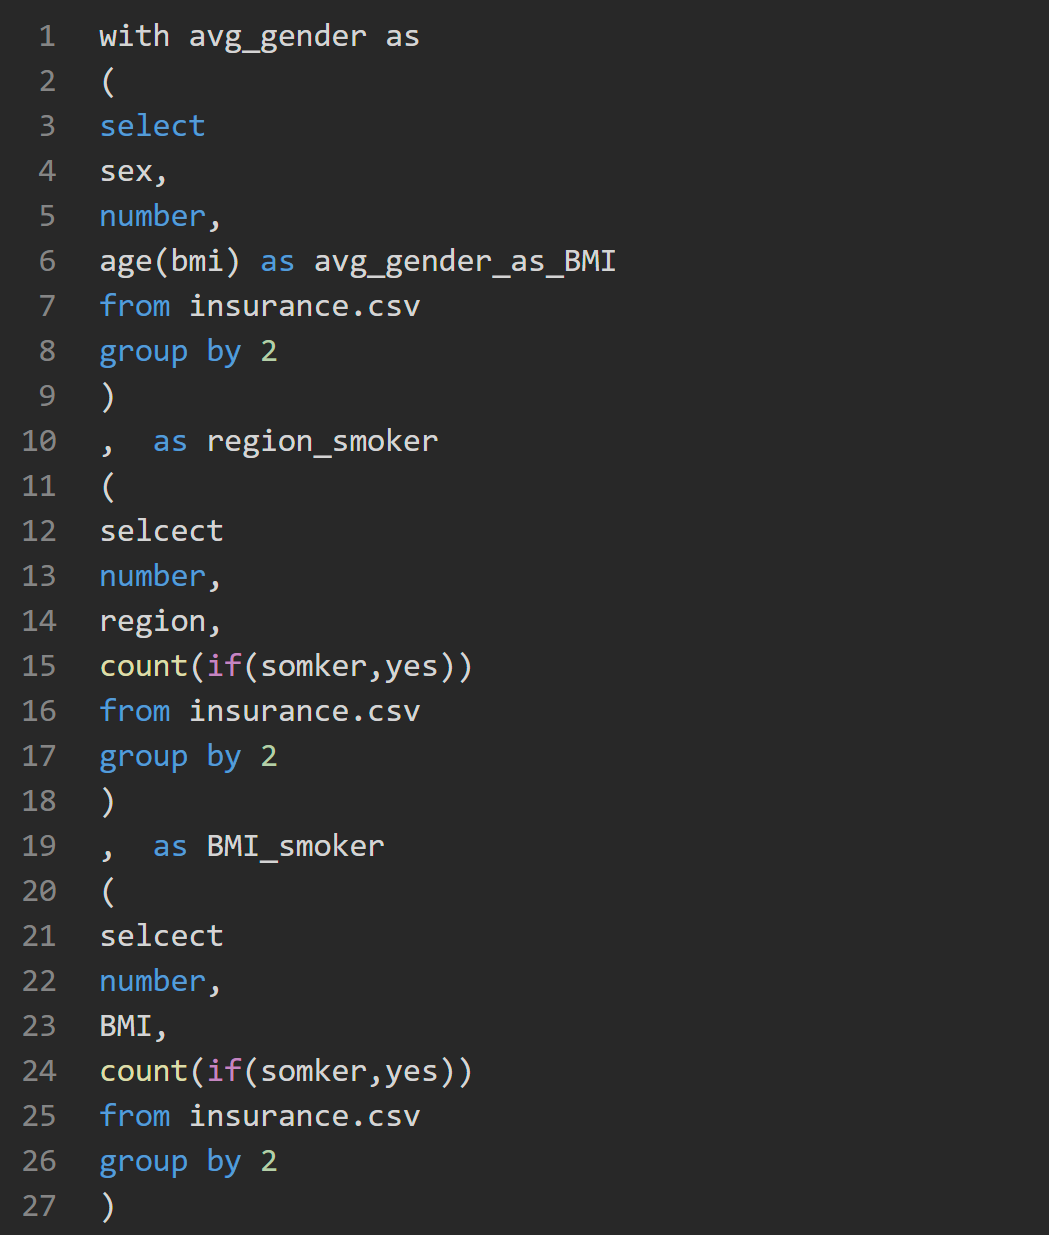
\includegraphics [width= 3.55 in]{13.png}
\caption{}
  \label{storage}
\end{figure}



 
 \par In most business situations where performance monitoring is needed, a lot of data needs to be imported, and the amount of table space needs to grow quickly. Data from the past should be cleaned up regularly so that disc space doesn't get used up and so that SQL execution works better[15]. Depending on how often data is collected and how long it will be kept, different timers can be set up in the application software to delete old data. This simple temporal cleansing procedure works well in the early stages of a business's launch. But the above-mentioned timer is likely to stop working as the organization grows, especially when a lot of data is coming in at once. Data can't be cleaned up, and since transactions keep table locks for a long time, flow control breaks down and the database stops. With a data description language and a language for data manipulation, SQL is based on relational algebra and tuple relational calculus. Data insertion, query, update, and deletion, database schema development and change, and data access control are all included in the scope of SQL. Although SQL is sometimes referred to as a kind of declarative programming, which it mainly is, it also has procedural programming components.

 \begin{figure}[h]
  \centering
  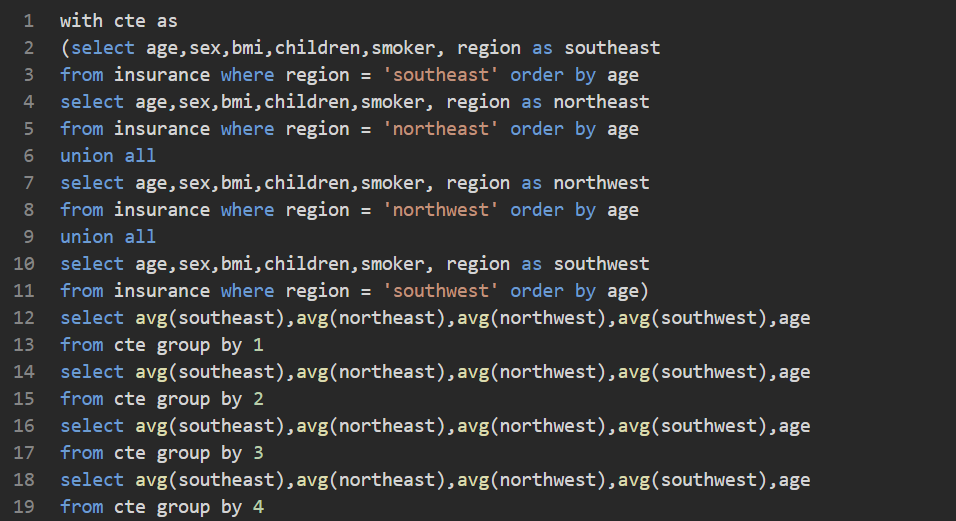
\includegraphics [width= 3.55 in]{sql.png}
\caption{During the data-calculating process, which also includes data cleansing, customers from various locations are accurately categorize and questioned. The data become more regular as a result.}
  \label{storage}
\end{figure}

Edgar Codd's relational model was first written in SQL, a commercial programming language, and was published in a major article in 1970. SQL, the most popular database language, was made even though it didn't follow Codd's relational paradigm perfectly. First, synchronous replication between Galera cluster nodes is mostly based on broadcast write sets and transaction verification. This is because they need to add things like multi-node simultaneous commit and conflict transaction rollback. Also, when the transaction is done on the local node, an optimistic method is used, and conflict detection happens after the message has been sent to all nodes[16]. The local transaction is reverted first when a conflict is found. If there are no conflicts, each node will run the write that was put in the queue at its own pace.

Even if the index is reached, the execution efficiency is very low, and it is simple to cause the system lock, as can be seen by looking at the execution plan. So, we need to suggest partition tables to really solve the problem of cleaning up data in very large tables. When data is deleted, it doesn't use DML operations; instead, it deletes the early partition tables (DDL) right away[17].
The write set only records the physical storage location of the table, its structure, and the constraints, triggers, indexes, and stored procedures that the table depends on when the drop operation is executed because the write set records the information of each row when the delete operation is executed. Using the drop operation is orders of magnitude faster when there is a lot of data in the table[18].
The fact that the application does not need to change the code is another benefit of the partitioned table. Setting up the back-end database and using the time field of the table as the partition field is an easy way to divide the table[19].

\begin{figure}[h]
  \centering
  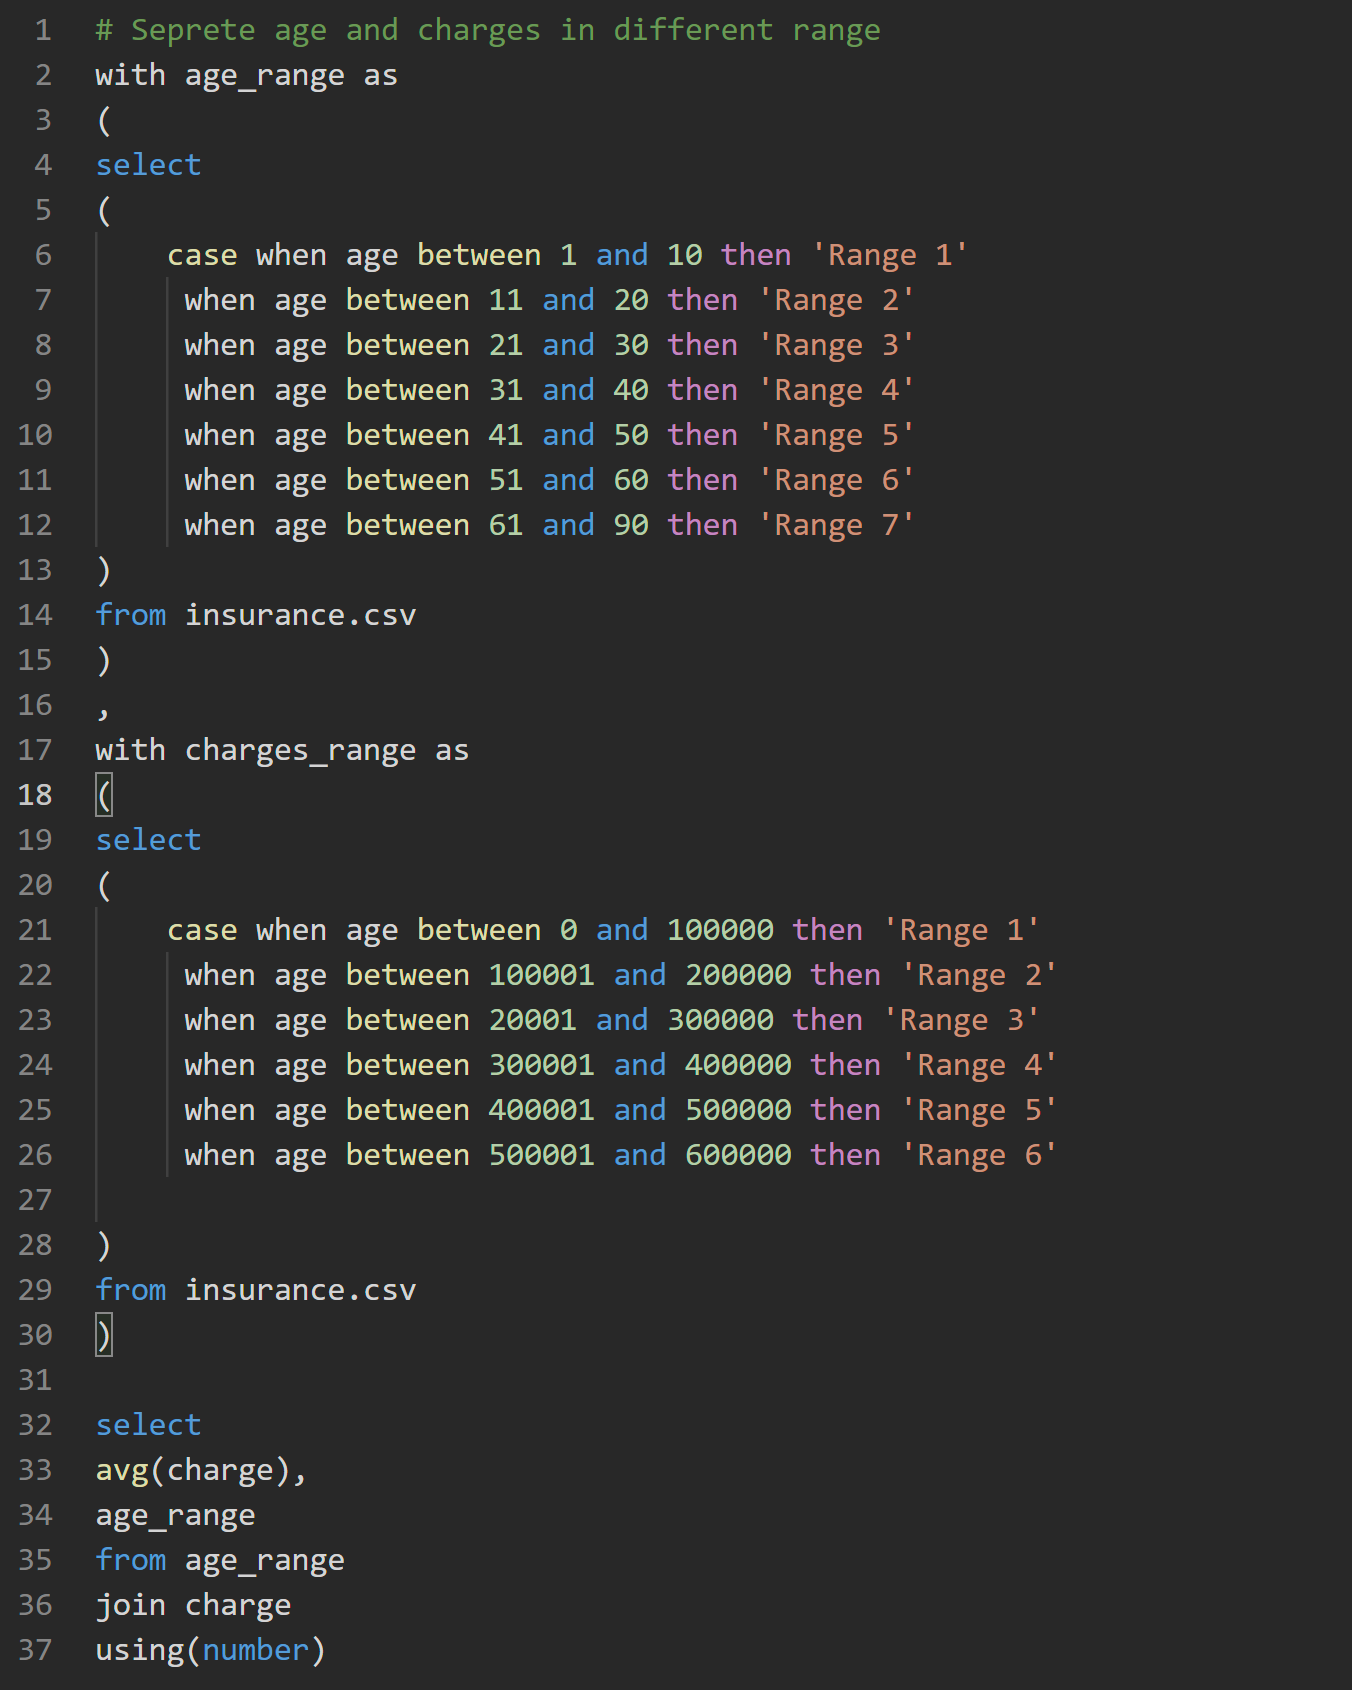
\includegraphics [width= 3.55 in]{12.png}
\caption{}
  \label{storage}
\end{figure}


 
\textbf{2.3 The Method of R}

\par It was first used in research and in the classroom. R is simple to obtain from CRAN (Comprehensive R Archive Network). More than 10,000 packages may be downloaded via CRAN, which can also be used as a package management. The R programming language may be used with well-known open source integrated development environments (IDEs), such R Studio. I agree that there are a lot of people on Stack Overflow who use the R programming language. Many of the questions I had about R when I was in college might have been answered in the Stack Overflow R language section. Online courses like Coursera provide beginning R and Python courses if you're just getting started with the languages. Both R and Python offer top-notch visualization libraries. Hadley Wickham, who is the Chief Scientist of R Studio, made ggplot2, which is one of the most well-known ways to show data in R. I adore ggplot2's numerous features and adaptability options. ggplot2 lets users customize charting elements in a more abstract way than standard R graphics. My favorite plots from the more than 50 offered by ggplot2 are calendar heatmaps, hierarchical treemaps, and cluster plots[20]. 

\begin{figure}[h]
  \centering
  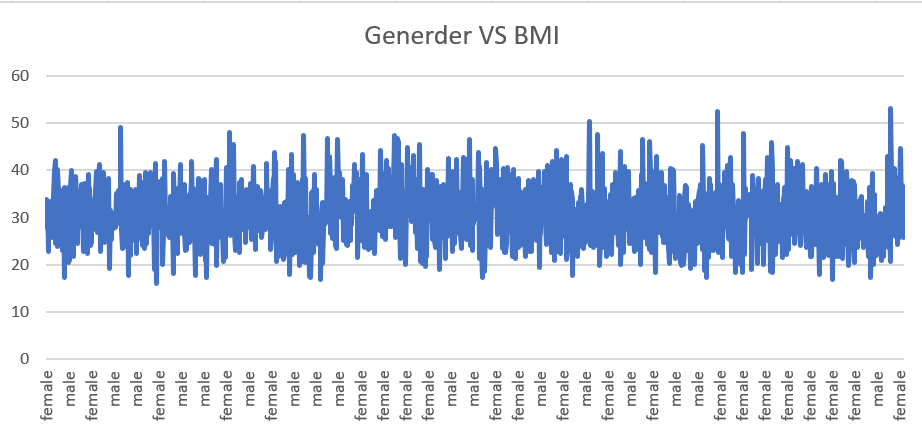
\includegraphics [width= 3.55 in]{1.png}
\caption{}
  \label{storage}
\end{figure}

\par R is a programming language and operating system for statistical computation and statistical graphics. It is free, open-source software. Even though it lacks C's flexibility and Perl's strong text processing features, the R language is great at computation, data processing, and graphics[21]. R makes it much easier for people who aren't computer majors to learn computer language. This means that statisticians who aren't computer majors can use computer language to do statistical work. The R language rose to popularity as a tool for data analysis. As more and more people with technical backgrounds join, the R language community keeps growing and getting bigger. In addition to statistics, the R language is now used in many other fields, such as education, banking, e-commerce, and the Internet. R was initially intended for statistical computing and illustration[22]. The R programming language can now do a lot more than what it was designed to do, such as data mining, machine learning, social networks, bioinformatics, financial data analysis, and so on. Since it is an open statistics programming environment, the syntax is easy to understand and easy to learn and master. After learning, you can create your own functions to add to the language that already exists. Because of this, it updates significantly more quickly than typical statistical software like SPSS, SAS, etc. Most of the most up-to-date statistical methods and procedures are available right away in R. A package's contents can only be accessible once it has been loaded. In the normal installation file, there are a few packages of regularly used and fundamental software. The software packages that are a part of the standard installation file are continually updated as new statistical analysis techniques are developed. The base-basic R module, the maximum likelihood estimation module (mle), the time-series analysis module (ts), the multivariate statistical analysis module (mva), and other packages are already in the other installation file. Its input and output windows are all carried out in the same window, with the exception of the graphics output, which is in a separate window[23]. The prompt will appear right away if there is a syntactic mistake in the input. It can be used at any time and remembers the instructions you've already given. Replicate, edit, and alter to satisfy user requirements. The images that are made can be saved right away as PDF files, JPG, BMP, PNG, and other image formats[24]. Additionally, there are effective interfaces with databases and other programming languages.

\begin{figure}[h]
  \centering
  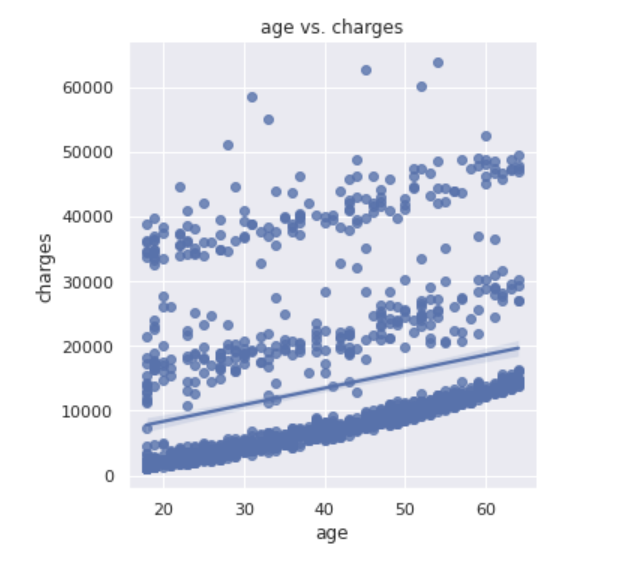
\includegraphics [width= 3.55 in]{4.png}
\caption{}
  \label{storage}
\end{figure}



\begin{figure}[h]
  \centering
  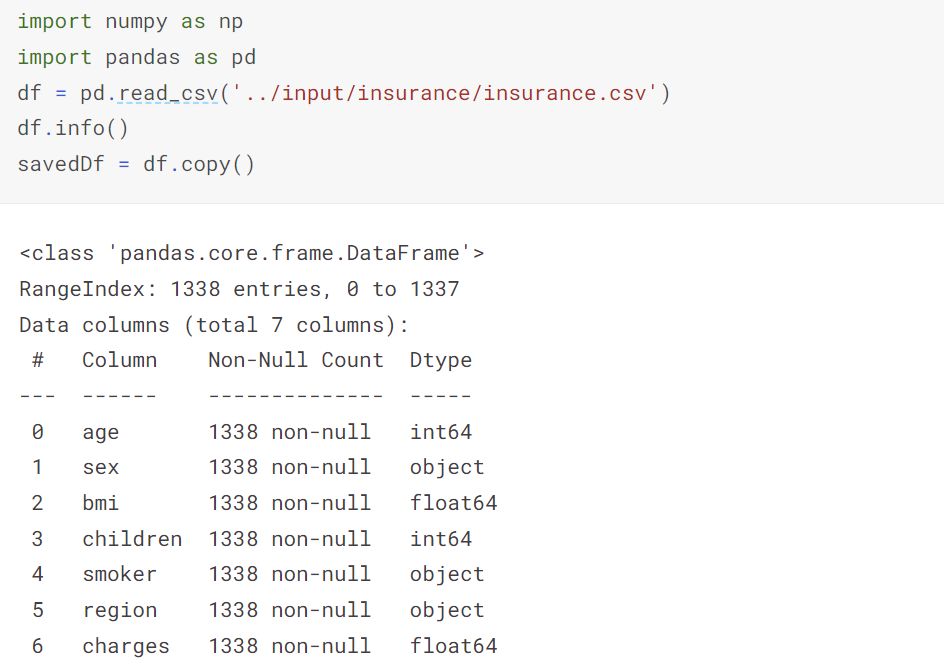
\includegraphics [width= 3.55 in]{7.png}
\caption{}
  \label{storage}
\end{figure}





\begin{figure}[h]
  \centering
  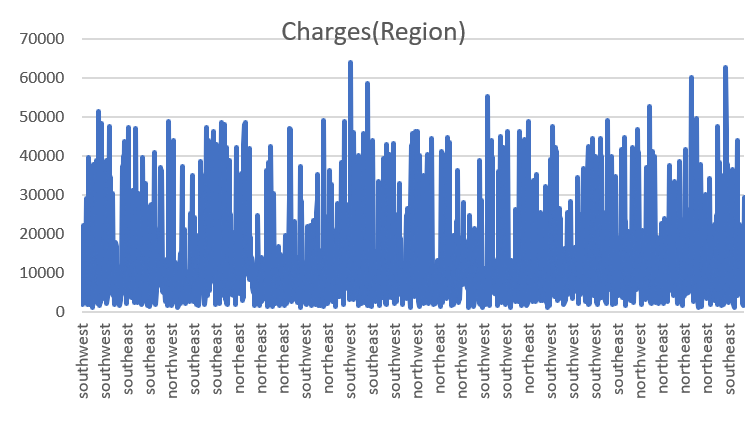
\includegraphics [width= 3.55 in]{2.png}
\caption{}
  \label{storage}
\end{figure}



\begin{figure}[h]
  \centering
  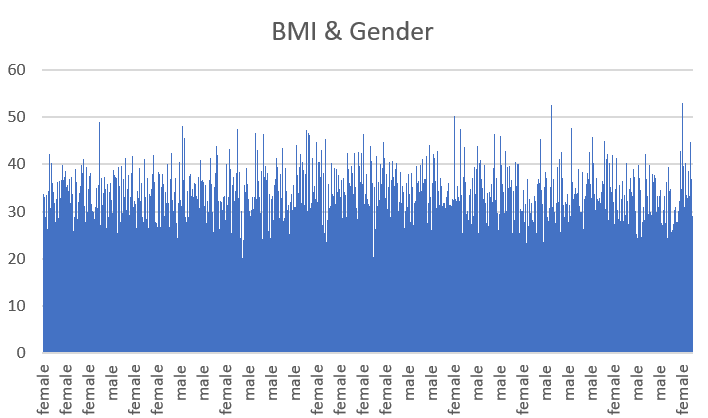
\includegraphics [width= 3.55 in]{3.png}
\caption{}
  \label{storage}
\end{figure}


\par These graphics are appropriate for a range of businesses. In terms of ggplot2 use, SelvaPython also offers a top-notch data visualization package. For creating and displaying statistical graphs, Matplotlib and its Seaborn extension are helpful. To learn more about visualization and have a better knowledge of Matplotlib, I suggest reading George Seif's paper. Follow Prabhakaran's excellent instructions. Both Python and R include robust libraries for predictive analytics. The effectiveness of the two in high-level predictive modeling is difficult to compare. Since R was made to be a statistical language, search and statistical modeling are easier in R than in Python. Programming language speed measurements are frequently skewed. Each language has built-in optimizations for certain tasks. For example, R is good for statistical analysis. There are several methods for performance testing in Python and R.Only the core distinctions between Python and R are covered in this article. Personally, depending on the work at hand, I would either choose Python or R. Data scientists have recently had trouble combining Python and R. There is a strong likelihood that a third language may appear soon and surpass Python and R in popularity. As data scientists and engineers, it is our job to keep up with technological changes and come up with new ideas[25].


\textbf{2.4  Data Collection }

\par Data mining is a type of analysis that uses computers to look at and learn more about huge amounts of data. Businesses may find hidden patterns and correlations in their data by using data mining tools and techniques. Data mining transforms unstructured data into usable information. Businesses use this information to solve problems, predict how their actions in the future will affect their profits, and increase their profit margins. Any good analytics program must include data mining. Businesses can use the knowledge discovery process to increase consumer trust, build customer loyalty, and find new ways to make money. All facets of corporate planning and operational management are aided by efficient data mining. Here are some instances of data mining's application across several sectors. Large client databases maintained by retail businesses include unprocessed information on consumers' purchasing habits[26]. These data may be processed by data mining to produce pertinent insights for advertising campaigns and sales projections. By using more accurate data models, retail businesses can improve customer happiness by making their sales and logistics work better. For example, data mining could show what popular seasonal items can be stored ahead of time so that there aren't as many shortages in case of an emergency. Because data mining software needs high-quality data, data miners spend the most effort at this phase. Business processes collect and store data, but not just for data mining. Before data miners can use it for modeling, they have to optimize it. These steps are included in data preparation. After entering prepared data, data miners use data mining tools to analyze the results. They can select from a range of data mining strategies and tools to do this. To figure out how good the results of data mining are, they also have to make tests. After the model has been made, the data miner starts to compare it to the business goals that were set up front. With business analysts, they discuss findings and gather comments. The model could give a good answer to the original question or show new patterns that had not been seen before. Based on what the company tells them, data miners may change models, change business goals, or look at data. The knowledge discovery process includes ongoing review, criticism, and correction. Association rule mining is a way to find connections between two different datasets that don't seem to be related. If-then clauses show how likely it is that two pieces of information will be related. Data scientists assess the correctness of outcomes using support and confidence criteria. Support is a measure of how often the relevant element appears in the dataset. Confidence is a measure of how often the if-then statement is true.

\begin{figure}[h]
  \centering
  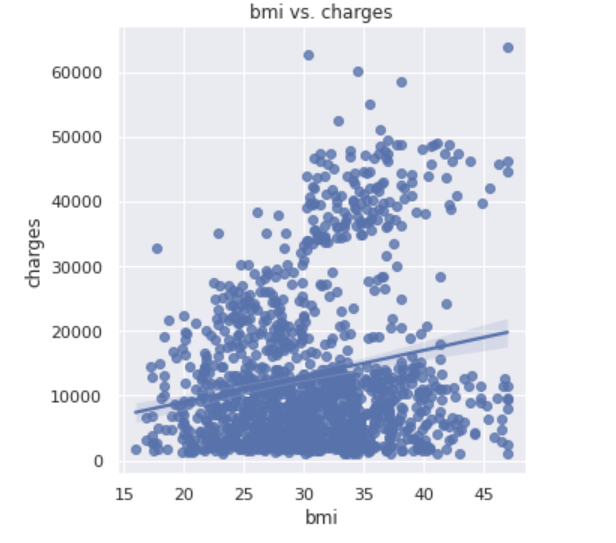
\includegraphics [width= 3.55 in]{5.png}
\caption{}
  \label{storage}
\end{figure}


\par For instance, clients frequently purchase a second, similar item along with a single one. By mining prior purchase data, retailers may discover new client interests. Findings from data mining are used to fill in the recommendations section of an online store. Classification, a complex data mining process, is used to teach ML algorithms how to divide data into different groups. To choose categories, it employs statistical techniques like closest neighbors and decision trees. All of these methods use pre-programmed algorithms to figure out what kind of data a new piece of data is based on how other data has been classified.

For example, researchers can use photos of apples and mangoes with notes on them to teach data mining tools what to look for. Using a new picture, the programm can correctly identify if it is an apple, mango, or another fruit.
Multiple data points are grouped via clustering according to how similar they are. It varies from classification in that it looks for patterns in data based on similarities rather than categorizing data according to particular categories. The result of data mining is a group of groups called "clusters." Each group is different from the others, but the things in each share some characteristics.


When dealing with multivariate survey data, for instance, cluster analysis might be helpful in market research. Researchers in the market use cluster analysis to divide customers into different groups and figure out how the different groups are related. Data mining tools can also seek for patterns in particular occurrences or collections of values that influence later occurrences. It can spot data changes that happen often or data points that fluctuate over time. For instance, a company may use route analysis to find that sales of particular items peak before the holidays or that warmer weather encourages more people to visit its website. Business intelligence is used in predictive data mining to identify patterns. Business leaders can use it to figure out how their actions will affect the future of the company and make wise decisions. For instance, a business may use information on previous product returns to create a warranty that doesn't result in a loss. They come up with a one-year warranty plan that takes into account losses when figuring out product prices and uses predictive analytics to estimate how many returns will be made in the next year.

 \begin{figure}[h]
  \centering
  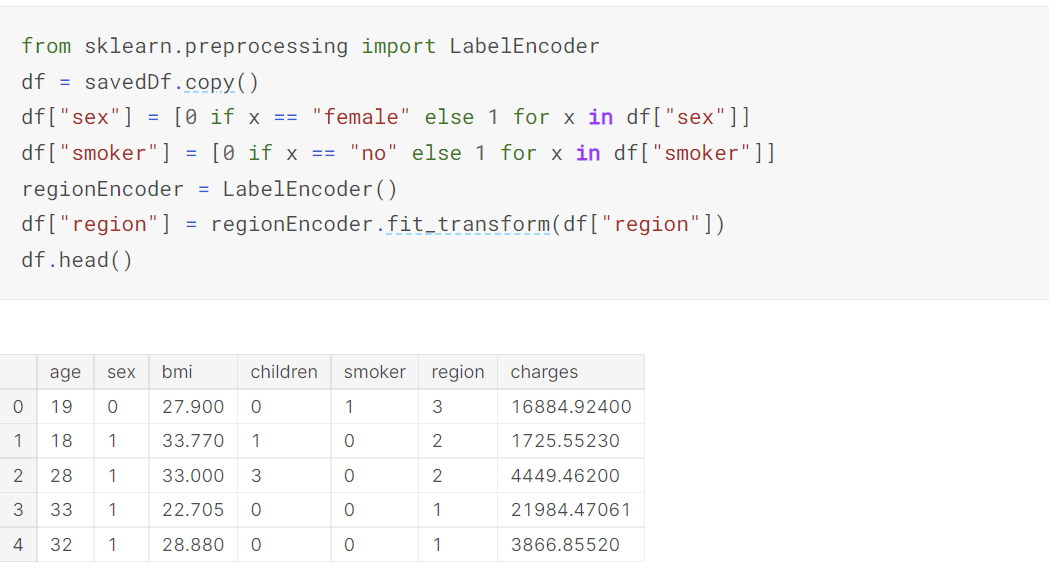
\includegraphics [width= 3.55 in]{6.png}
\caption{}
  \label{storage}
\end{figure}

\section{Result and Discussion }

\textbf{3.1 Data Analysis}

\par In order to optimize the growth of data functions and play the role of data, "data analysis" refers to the application of suitable statistical analysis methods to evaluate a significant quantity of gathered data, and summarize, interpret, and digest them. Data analysis is the process of carefully reviewing and summarizing data in order to draw conclusions and extract relevant information. Data analytics is used to turn unprocessed data into knowledge that can be put to use. It has a variety of tools, methods, and steps for using data to find patterns and solve problems. Data analytics may influence how businesses operate, enhance decision-making, and promote expansion. Companies can better understand operations and services thanks to data analytics[27]. It gives businesses an in-depth understanding of client problems and experiences. Companies may develop tailored consumer experiences, construct pertinent digital services, optimize processes, and boost staff productivity by shifting the paradigm from data to linking insights to action. A data warehouse is a database made for analyzing relational data from corporate applications and transactional systems. Pre-defined data structures and schemas are optimized for quick searching and reporting. Data is cleaned, improved, and changed so that consumers have a "single source of truth" that they can trust. Customer profiles and product information are two examples of data.

 \begin{figure}[h]
  \centering
  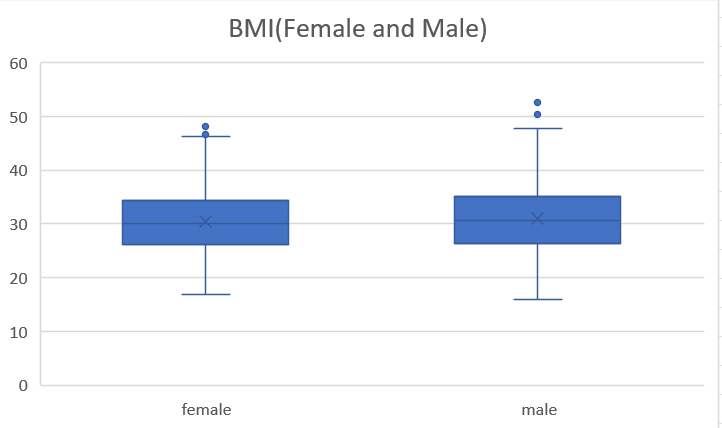
\includegraphics [width= 3.55 in]{8.png}
\caption{}
  \label{storage}
\end{figure}



\par The difference is that a data lake can store both structured and unstructured data without having to do any extra work. Since the structure or schema of the data is not known when the data is collected, any data can be stored without a lot of planning. This is especially helpful when it's not clear how the data will be used in the future. Social media content, IoT device data, and non-relational data in mobile applications are a few examples of data. Businesses can hire outside assistance to evaluate the data. When management and executive teams outsource data analytics, they are free to focus on other important business tasks. Professional business analysis teams are the best at what they do, know the newest ways to analyze data, and are skilled at managing data. As a result, they can analyze  data more quickly, spot patterns, and accurately forecast emerging trends. Outsourcing, on the other hand, can cause problems for businesses in terms of data security and the transfer of knowledge. Marketing, product development, content production, and customer support are all simplified by data analytics. By examining real-time data, data analytics helps businesses to create tailored content and perfect it. Data analytics can also provide useful information about the effectiveness of marketing campaigns. Based on real-time information, businesses may fine-tune objectives, marketing, and creativity. Analytics can improve marketing to boost conversions and cut down on wasteful advertising. Data analytics is used by businesses to prioritise new features and find new features for product development. They can figure out what consumers want, give them more features in less time, and make new products available faster. Many data tasks, like data transfer, preparation, reporting, and integration, can now be done automatically thanks to data analytics. It eliminates the inefficiencies of manual procedures and cuts down on the amount of time and labour needed to manipulate data. Scaling is supported by data analysis, enabling you to easily implement new concepts. Businesses collect quantitative data, statistics, and information from several internal and customer-facing channels. Finding important insights, however, necessitates the rigorous examination of enormous volumes of data. This is not a simple job. Look at some examples of how data science and analytics have benefited organizations. Marketing, product development, content production, and customer support are all simplified by data analytics. By examining real-time data, data analytics helps businesses to create tailored content and perfect it. Data analytics can also provide useful information about the effectiveness of marketing campaigns. Based on real-time information, businesses may fine-tune objectives, marketing, and creativity. Analytics can improve marketing to boost conversions and cut down on wasteful advertising.

\begin{figure}[h]
  \centering
  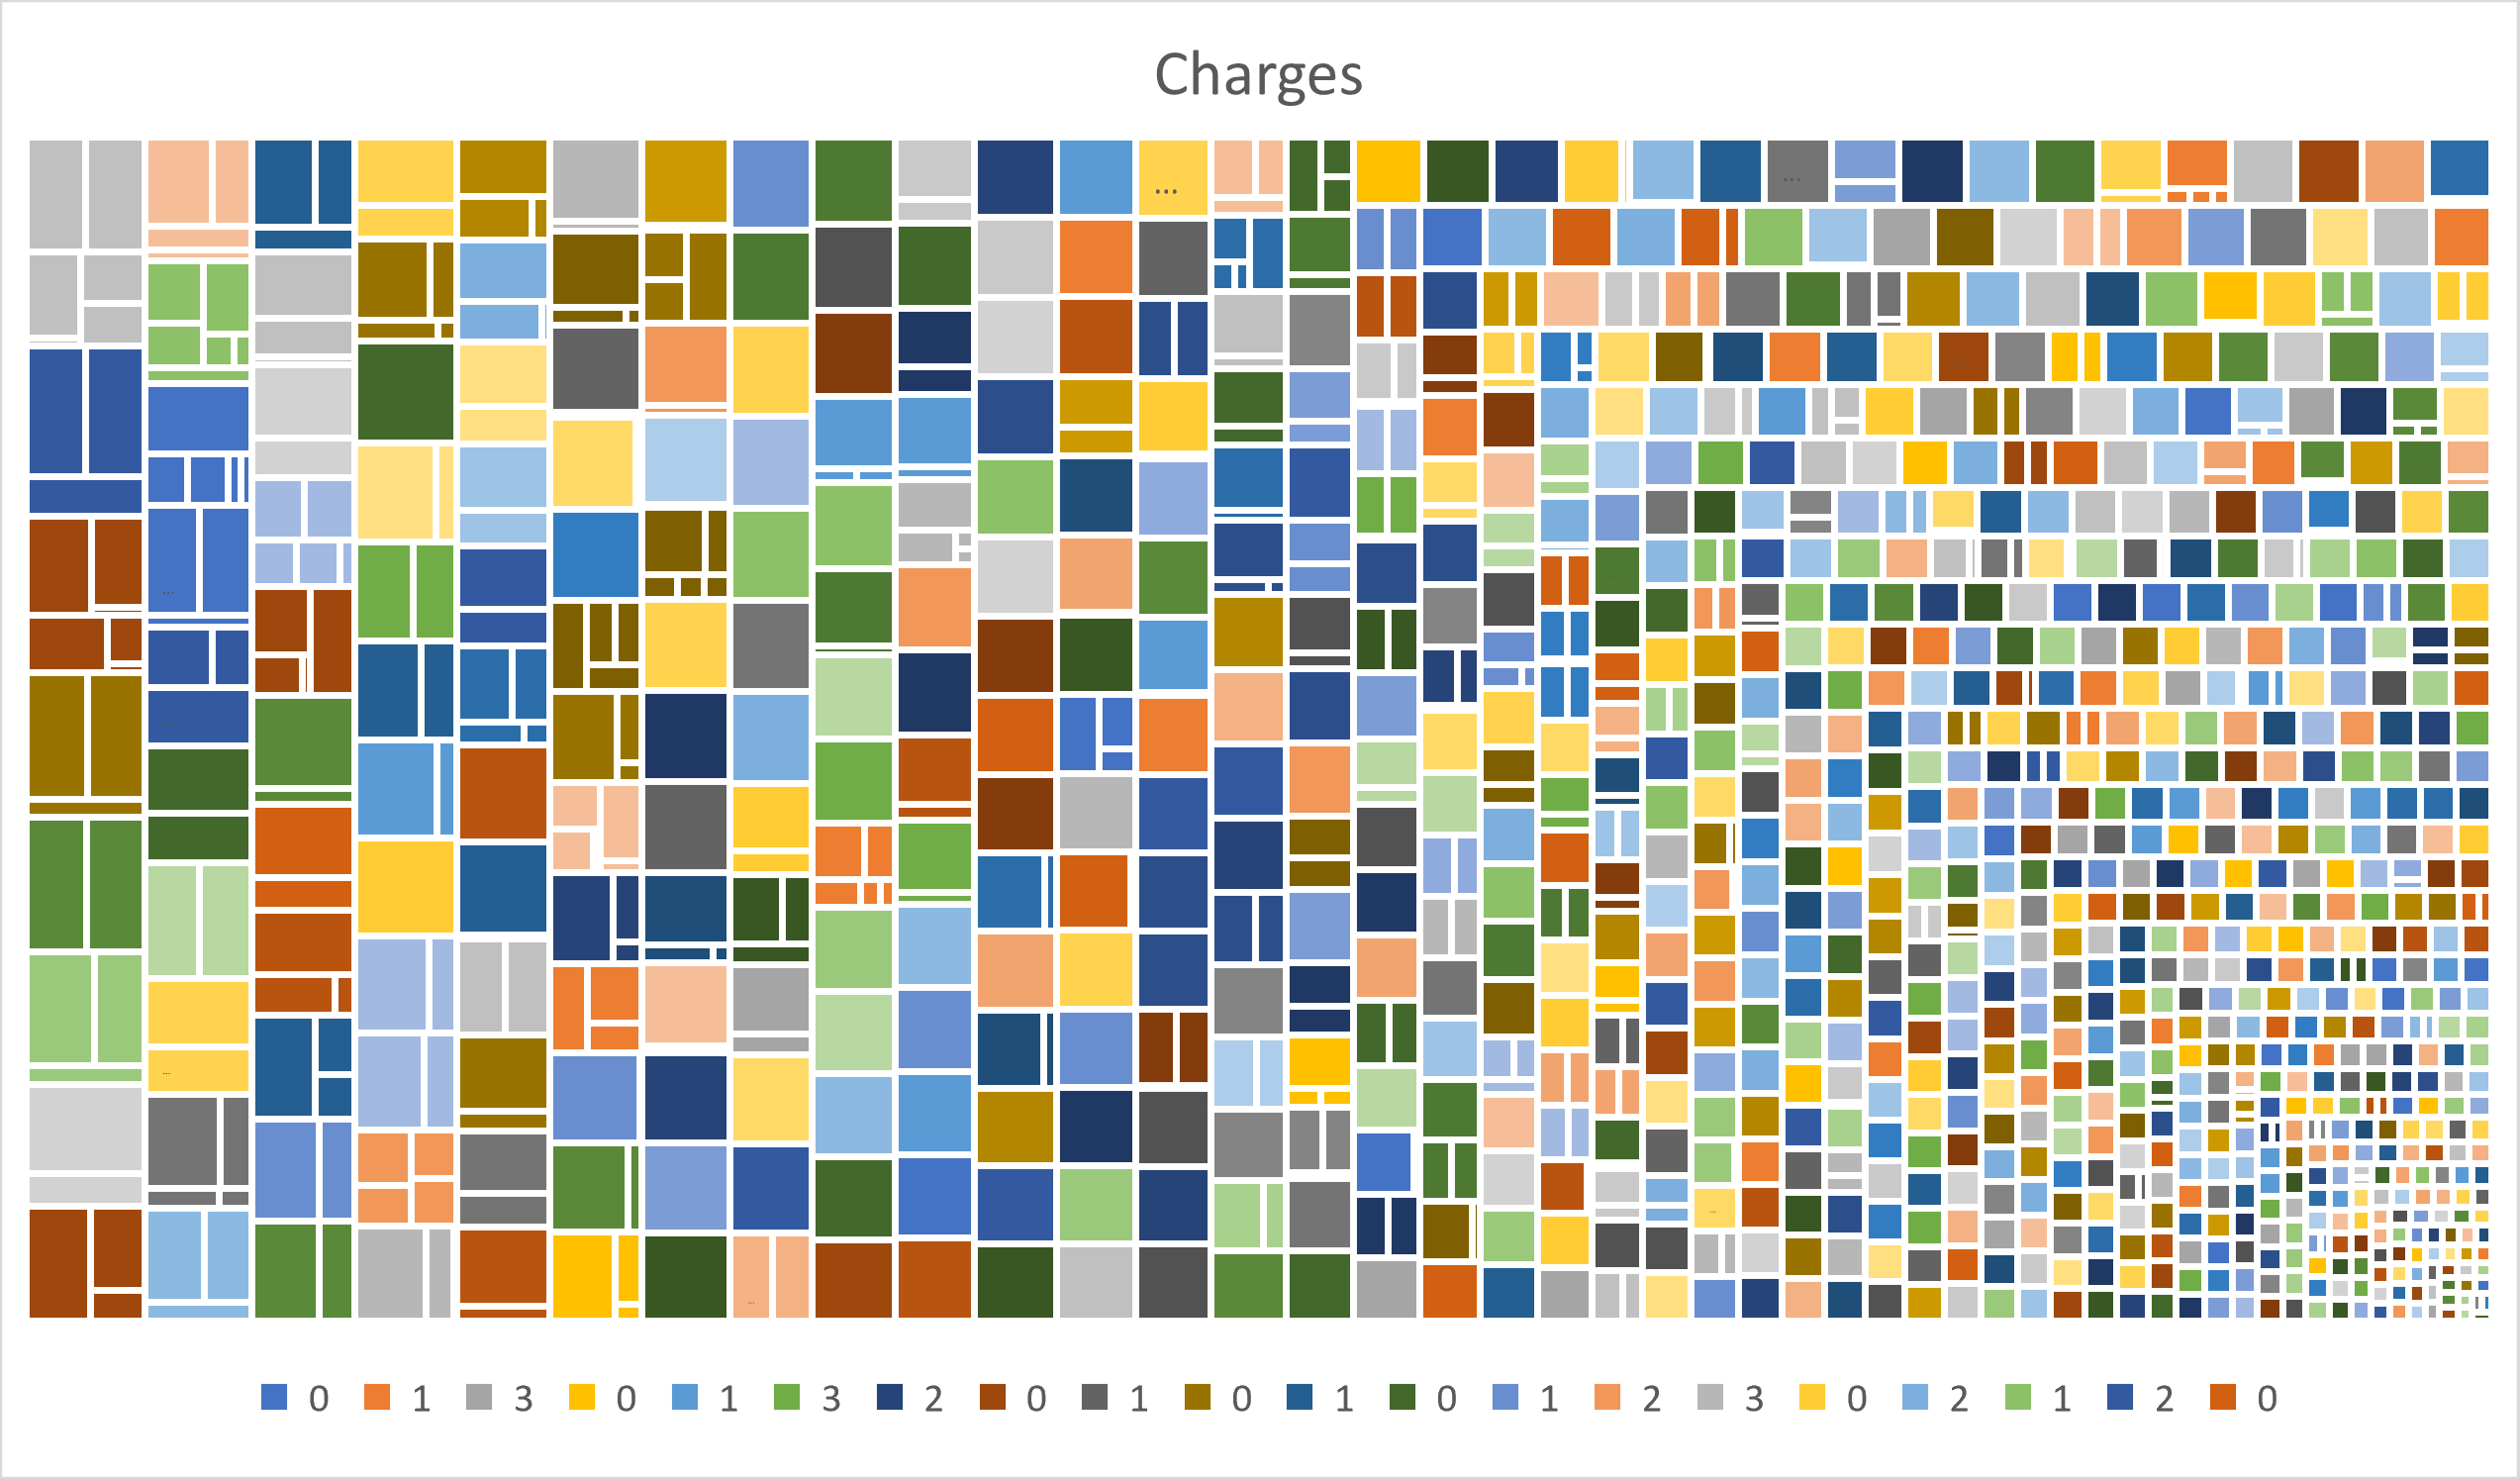
\includegraphics [width= 3.55 in]{11.png}
\caption{}
  \label{storage}
\end{figure}

\par Data analysis is more likely to identify solutions to practical issues than data mining, which looks for relationships, categorization, and clustering. What choices am I able to make based on this analysis? The goal of data analysis is quite powerful, for instance, when deciding whether to organise an event at a specific institution or whether to expand our subsidy programme by another 10 yuan. The initial distinction between data analysis and data mining is the source of the data. As long as the information is relevant to the analysis aim, it may be acquired from a variety of sources, including databases, information collecting forms, visits, and other types of data. The reading of database data is skewed in data mining. The data for data analysis is more disordered as compared to data mining, which derives its data straight from the database. You can look for data on Baidu or in the analysis reports of other individuals. These data have distinct fields and formats. Not united, you must categorise and integrate here in accordance with your goals. The most crucial step in the entire process is data analysis! The most crucial thing here is to constantly consider your aim. For instance, you must compare year over year, month over month, etc. in order to comprehend the transaction status over a specific time period. There are several approaches and materials in this field. I won't go into great detail here because the topic only wants to grasp what data analysis is. Your results are explained in the data report! To demonstrate your professionalism, you can create a tonne of complicated formulae. In this area, data scientists are continually developing. These experts analyse data using various forms utilising techniques including data mining, data management, and statistical analysis. Structured, semi-structured, and unstructured data are meticulously extracted and cleaned in these jobs. They employ data visualisation to convey their results after discovering actionable insights, which enables stakeholders to quickly absorb the new knowledge. To produce important new directions and breakthroughs across many sectors, each stage of the process is essential.

\par Each of these applications fits under one or more of the following categories: prescriptive, diagnostic, descriptive, and online, albeit the precise methodology for data analysis differs depending on the application. Prescriptive analytics: Prescriptive analytics, like current iterations of predictive analytics, can offer the best suggestions depending on the circumstance in real time. Diagnostic analysis: This sort of analysis use methods like drill-down, correlation, and data mining to ascertain the reasons behind occurrences, spot trends, and take prompt action. Similar to diagnostic analytics, descriptive analytics sifts through past data to help provide fresh viewpoints. However, descriptive analytics employ techniques like statistics, clustering, and segmentation to build a more complete picture of what happened rather than offering a justification for why an event occurred. Predictive analytics: As the name implies, this methodology forecasts future events using data from several sources, including statistics, modelling, data mining, machine learning, and other types of data. Cyber analytics is a more recent type of analytics that combines data science and cybersecurity principles to find possible security holes and active cyberthreats. Anyhow, a data scientist will make use of whatever platforms and analytical tools are now accessible to help him analyse the topic he is attempting to answer.





\textbf{3.2 Result}
\par Analyzing data trends to obtain information and insights to improve decision-making is known as data analytics. Both non-technical folks and data analysts and scientists work together to complete this difficult task. The process frequently begins with raw data, which is then mined for insightful information; in fact, the main objective of corporate data analytics is to gain a competitive edge.
The reason why the concept of data analytics hasn't evolved as much as some other technical definitions is mostly because experts generally concur that data analytics encompasses practically anything a company might accomplish with raw data. For instance, data analytics is described by Gartner as "the management of data for all purposes (operational and analytical) and the analysis of data to drive business processes and improve company results through more efficient decision-making and increased customer experience. Data mining is the process of turning unprocessed data into knowledge that businesses can use. The most popular approach is to use various data mining technologies to detect patterns in the data. Data analysis includes data mining as a subset. Additionally, data mining combines machine learning and artificial intelligence. the main building block of the Over time, several methods for using and practising data mining have been created. Each method expands on the basic concept of finding patterns in a set of data. The project's aim and the breadth of the investigation can both influence how the data is continually improved. For instance, correlation may be used to simply correlate a large number of dependent variables, outliers and anomaly identification can be used to dig down and comb through big datasets in search of any oddities, and so on. A data lake is a storage space where massive volumes of unprocessed raw data are kept until they are needed. A data lake is a flat file format that maintains the original structure of the data as it is input, in contrast to structured data warehouses, which employ hierarchical data structures like folders, rows, and columns. Each data piece has a specific identification assigned to it and is also given an extensive variety of metadata tags. All tagged data is examined for query or analysis when a business query based on a certain metadata is run. Data lakes were created because people needed a place to store all of the information they were gathering from the Internet of Things and other sources. Relational databases serve as the historical store medium. However, these technologies are crucial for us to gather data from all around. Not true for all of these bits of information. Data grids are becoming more popular as a tool to assist businesses better manage their dispersed processing needs, quickly expanding data quantities, and changing application requirements. Data grids might be thought of as It links various on-premises and public cloud locations, kinds, and sources of data as a network spanning a broad network, and it makes use of those connections to process, transfer, manage, and store data throughout the fabric. Applying structures and procedures to data is the act of transforming it into a form that can be used for analysis and insight. It is feasible to optimise database design and comprehend information system problems by creating the data models used in information systems. flow of data A good data model is an abstract representation of the specifics of the database, including how data is collected, how it moves through the system, how it is put into different tables, and what validations and constraints are used before the data is saved in the database.


  \begin{figure}[h]
  \centering
  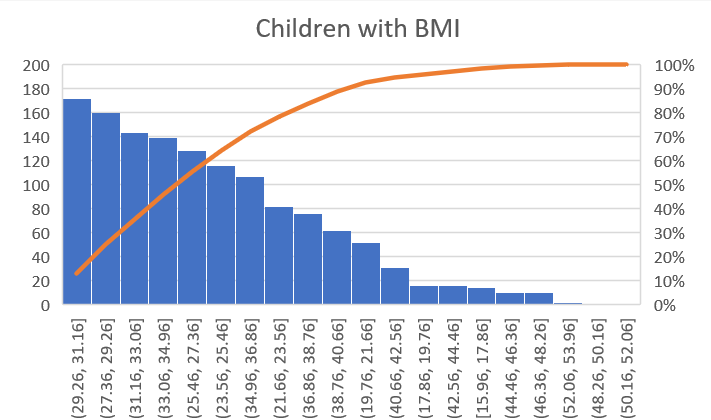
\includegraphics [width= 3.55 in]{9.png}
\caption{}
  \label{storage}
\end{figure}

\par Devices can now analyse information for contextual analysis and action thanks to advances made in deep learning, an artificial intelligence technology that mimics certain characteristics of the human brain. Deep learning adds multilayer neural networks to machine learning (ML) methods to make decision trees with many layers that link decisions and variables that are related. Moving ahead in the self-driving car example results in judgments regarding speed, whether to avoid obstacles, finding a destination, and other matters. These following choices, however, can result in feedback that makes the AI reevaluate and alter past choices. For us to learn, we need to be told what to do and make several decisions almost at the same time. Deep learning seeks to replicate the human brain. Research and development, engineering, and strategic planning all depend on data analysis. Of course, it is the foundation of supply chain and logistics management. Analytics are becoming more and more important in information technology and cybersecurity every year. Overall, data analytics are scarcely present in any sector of the economy. Today, many companies have a chief data officer whose responsibility it is to handle all facets of data management, including data analytics and data science. Thorough examination Descriptive analysis explains what has already occurred or is occurring right now. Who, what, where, when, and how are just a few of the issues this kind of research may address. Examples of descriptive analytics include a sales report that shows monthly sales for the last four quarters. Although it is the simplest sort of analysis to do, it is not particularly useful to a company. Descriptive analytics, on the other hand, can't be ignored because they are the building blocks for more advanced analytics. You can find out why something happened through diagnostic analysis. For instance, diagnostic analytics may be used to determine what went wrong if descriptive analytics reveals that sales decreased last quarter. This kind of study frequently combines many data sources to produce a more thorough and precise evaluation of the state of an organization. Sales may be down as a result of weather conditions, supply chain problems, or the loss of a major client following the hire of a new salesman. Diagnostic analysis can be used to solve this. The use of predictive analytics enables you to anticipate potential outcomes. It examines patterns in previous trends to get insight into the future. Advanced data models and machine learning are often used by predictive analytics systems to find and use the key factors that affected past performance. This is a more sophisticated and speculative type of study that has a lot of promise. It is quickly becoming a highly popular tool, especially for big businesses. Prescriptive analytics try to tell you what to do about things that might happen in the future. Predictive analytics, for instance, might assist in understanding how things might change if pricing is dropped, marketing techniques are altered, or items are purchased from other suppliers if predictive analytics indicates that sales will decline in the upcoming quarter. Prescriptive analytics has a lot of potential benefits, but it's also hard to do it right. Few businesses have the tools and skills they need to use prescriptive analytics on a large scale right now. Descriptive analysis is often how most businesses begin their data analysis. They eventually grew to include diagnostic and later predictive analytics. Achieving a successful prescriptive analytics program is a goal shared by many who want to make better business decisions.

\par Most experts agree that data analytics is important for modern businesses because it makes them more competitive. Forrester says that "data is essential to improving the customer experience and operational efficiency, which in turn contributes to the success of a company." Sound data analysis is essential for realizing all of data's potential. There are several reasons why businesses do data analytics and analyze their data. program in science. Utilizing data analytics, you can accomplish a variety of tasks, including: Most businesses have access to a lot of information about their customers, such as demographics, purchase histories, interactions with customer service reps, social media, browser histories, survey results, and more. By hiring a data analyst to look at this information, businesses may be able to learn more about each customer and their customer base as a whole. It could also show ways to reach out to new groups of customers or better meet their needs. A business has many processes, such as taking orders, filling them, managing the supply chain, helping customers, running IT operations, and more. is quantifiable. Everything that is measurable may be made better. Key performance indicators (KPIs) may be tracked over time, and data analytics can help find bottlenecks that are currently holding down enterprises.
\par Gap analysis is one of the most fascinating subfields in data analysis. This process helps companies find projects they aren't working on right now but might be in the future. It may aid in locating new clients, merchandise, and partners, boosting sales and profitability. Even with the most basic data visualizations, it is easy to observe the direction and pace at which KPIs are changing. You may do more of the things that work well and attempt to fix the things that go wrong by finding these patterns, which often requires sorting through raw data. Marketing is one of the areas of business where data analytics have had the most impact. Because digital marketing is so common, marketing teams now have access to a lot of data that can be used to figure out which prospects are most likely to become customers, which customers are most likely to buy again, which customers are most likely to switch to competitors, and more. Data visualization is often used to support data mining for business insights. What if a price increase resulted in a  rise in an organization's total profit? You may examine the factors with the help of analytics. Pricing teams may use data analytics to help them decide where to raise prices (and where to cut them) in order to increase profits. People always act based on how they feel, which is often based on assumptions that may or may not be true. Data analysis is a strong way to fight this urge, so business leaders can figure out if their gut feelings are likely to work. In a broad sense, data analytics could help companies make better decisions across the board.

\section{Result and Discussion }

\par Because they lack a contemporary strategy to data and analytics governance, organizations trying to grow their digital company will fail. Other significant topics to keep an eye on include machine learning and artificial intelligence, in addition to data governance. Predictive and prescriptive analytics are two of the most advanced types of data analytics. Both rely on AI and machine learning skills. Analytics will become more powerful as a result of these technologies. artificial data. The amount of analysis a corporation may do directly on client data is often limited by privacy rules. One way to solve this problem is to use synthetic data that has been anonymized and is often specified by data models and algorithm development. various analytics centers and solutions. Most large businesses find that there is no one analytics solution that can meet all of their needs. Experts say that the most successful businesses are likely to be the ones that come up with creative ways to combine their many analytics solutions and data storage businesses. Long-term success is expected to favor organizations that keep up with these trends and those discovered via data analytics efforts.

\par The data processing approach is referred to as the "narrow method." It often has to do with statistics, measurements, modeling, and other methods used in economics, management, and other fields. When the word "methods" is used in a broad sense, it usually means normative analysis techniques or empirical analysis techniques that start with real-world events. The next phase for researchers to think about, with the goal issue in mind, is how to get the necessary data support. This comes after developing the analytical framework and choosing the theoretical foundation and model. The research's supporting data may be divided into two categories: statistical data and case data. Government and survey data make up the majority of the currently used databases for academic research (administration data). Survey data are usually the information that academic institutions, scientific research organizations, and other groups collect in order to do certain kinds of research. Currently, certain frequently used database resources exist in related fields, including economics and management. The majority of these data sources are micro-level data, such as pertinent information on people, families, businesses, etc., which have the characteristics of big samples, many variables, lengthy time periods, and rigorous research techniques. These databases could help researchers save money on research, make their research more effective, and come up with new research ideas. Researchers also get a lot of empirical data from government data, which is mostly macrodata like census data from the National Bureau of Statistics or data from demographic or agricultural censuses.
\par These days, it's incredibly straightforward to receive such information on the Internet. The CNKI China Economic and Social Big Data Research Platform is a common source of data. This portal has all of China's national, provincial, and major prefecture-level statistical data and yearbooks from all departments. It can do things like analyze data from data mining, make online reports, show how indicators work, and navigate a yearbook. Additionally, websites like Guoyan.com and Soushu.com provide online macro data retrieval and presentation. Primary data might also be gathered by researchers based on their study objectives. It's mostly about getting information through surveys or tools like web crawlers. Questionnaires are a typical tool for gathering the data needed for empirical research. The primary goal of this strategy is to guarantee the accuracy of the data. Indicator design, sampling technique, sample size, survey method, questionnaire design, organizational strategy, and quality control are all things that need to be improved to make survey results more reliable and valid. The use of web crawler technologies to sort and filter Internet data is another important way to make research data sets. Internet data is made up of a huge number of samples that are spread out over many different websites and are often changed. Crawler technology may now be used to gather this data and compile it into a data set for analysis. The case study approach requires obtaining case data in order to substantiate its findings. It usually isn't in the form of data, but instead is written descriptions of one or more event processes that are important to the study topic. The sequence of events includes all of the information that supports this kind of research method. The process of gathering case data often includes pre-research, formal research, and making a plan for how to do research. Research program design is the logical link between research questions and real-world materials. This usually includes problem formulation, theoretical assumptions, analysis frameworks, definition of analysis units, formulation of research programs, etc., and forms a set of cases that can be used as a guide for case research. criterion for screening and gathering evidence. Case studies often filter possible instances based on their theoretical underpinnings and analytic routes. It is necessary to appropriately take into account the ease of case study in addition to the concepts of typicality and variety. Before doing formal research, you might do pre-research to see if the strategy will work. When choosing pre-research cases, it's important to think about how easy and typical they are, and the total cost of the study should be cut down as much as possible. At the case data collection stage, it's important to fully use a variety of sources of evidence and collect different types of supporting materials for the same problem. This will improve the reliability and validity of the research materials and prevent problems caused by information asymmetry in the investigation. Irregularities that are both subjective and objective, like being misled by respondents or ignoring the difference between how the policy is written and how it is actually put into practice, etc. So that evidence from different sources can be checked by each other, researchers should know about the many common sources of evidence in case studies and choose which kinds of materials to collect based on their research goals and the amount of data they have access to.


\textbf{3.3 Expect Contribution}
\par Establish the report's target audience and analytical goals. You must first determine who the report is for, regardless of the sort of data analysis report you are writing. An audience's expectations for a data analysis report might vary. A clear framework and clear thoughts are the most important parts of the result of a data analysis. In a good data analysis report, you should explain your ideas about how to analyze the data so that the reader can fully understand what you are saying. As a result, the structure and concepts of a report must be crystal clear. In this case, the framework is mostly about how the data analysis process is set up, not just how the report is written. For instance, it is hard to immediately identify the cause of an analytical issue. The analytical frameworks that we often discuss, such as MECE, PEST, and AAARRR, may be employed at this point. We need to apply a variety of methods to dismantle and analyze the issue. Ensure data precision
More than 60 of the time is often spent on writing, collecting, and arranging data for reports. Data planning, coordinating with pertinent departments to arrange data gathering, exporting and processing data, and eventually writing a report are all required. If the data is wrong, the analysis won't be useful and the report won't be worth much. Because of this, it is important to think about how reliable the data is as it is being collected and put together. Check the data range and data calibre using Spectrum. Let the charts speak more clearly. When creating data analysis charts, it's important to understand how to explain the connections between the charts and how to communicate the issues they represent. Many cautious leaders will be worried about your data analysis and findings because they care most about the present and the future. So, data charts shouldn't just be used to show facts. They should also show how you think about analyzing the facts.


\section{Conclusion }  
\par This part of a general article will quickly describe the analysis results (results, findings) with charts, evaluate the difference between the analysis results and the expected results around the key arguments and operational arguments, and suggest more research. Once the data analysis is finished, it is critical to explain the analytical findings in conjunction with the study goal, that is, the arguments that have been presented. Data analysis is solely used to determine if a value is statistically significant. An explanation of the significance of this value and the associated judgement must be provided by the researcher. To highlight the uniqueness and practical importance of the arguments made in the conclusion section of the thesis, it is vital to choose relevant reference points throughout the explanation process, such as prior views or practises on the subject or findings from related research. The conclusion should be one of the six parts of the thesis research project. It should be different from the study plan. However, the research's major purpose when it comes to the conclusion is to represent the issue. Here, the key ideas that need to be emphasized in the conclusion section are summarised in a single section. A subset of advanced analytics called predictive analytics uses historical data together with statistical modelling, data mining, and machine learning to forecast future results. Businesses use predictive analytics to look at this data and find trends, risks, and opportunities.

\par Big data and data science are often linked with predictive analytics. Data from transactional databases, equipment log files, photographs, video, sensors, and other sources are all around businesses nowadays. Data scientists employ deep learning and machine learning algorithms to find patterns in this data and anticipate what will happen in the future. There are both linear and nonlinear regressions, as well as decision trees, neural networks, support vector machines, and more. Prescriptive analytics may further leverage the findings from predictive analytics to support actions based on predicted insights.

\begin{figure}[h]
  \centering
  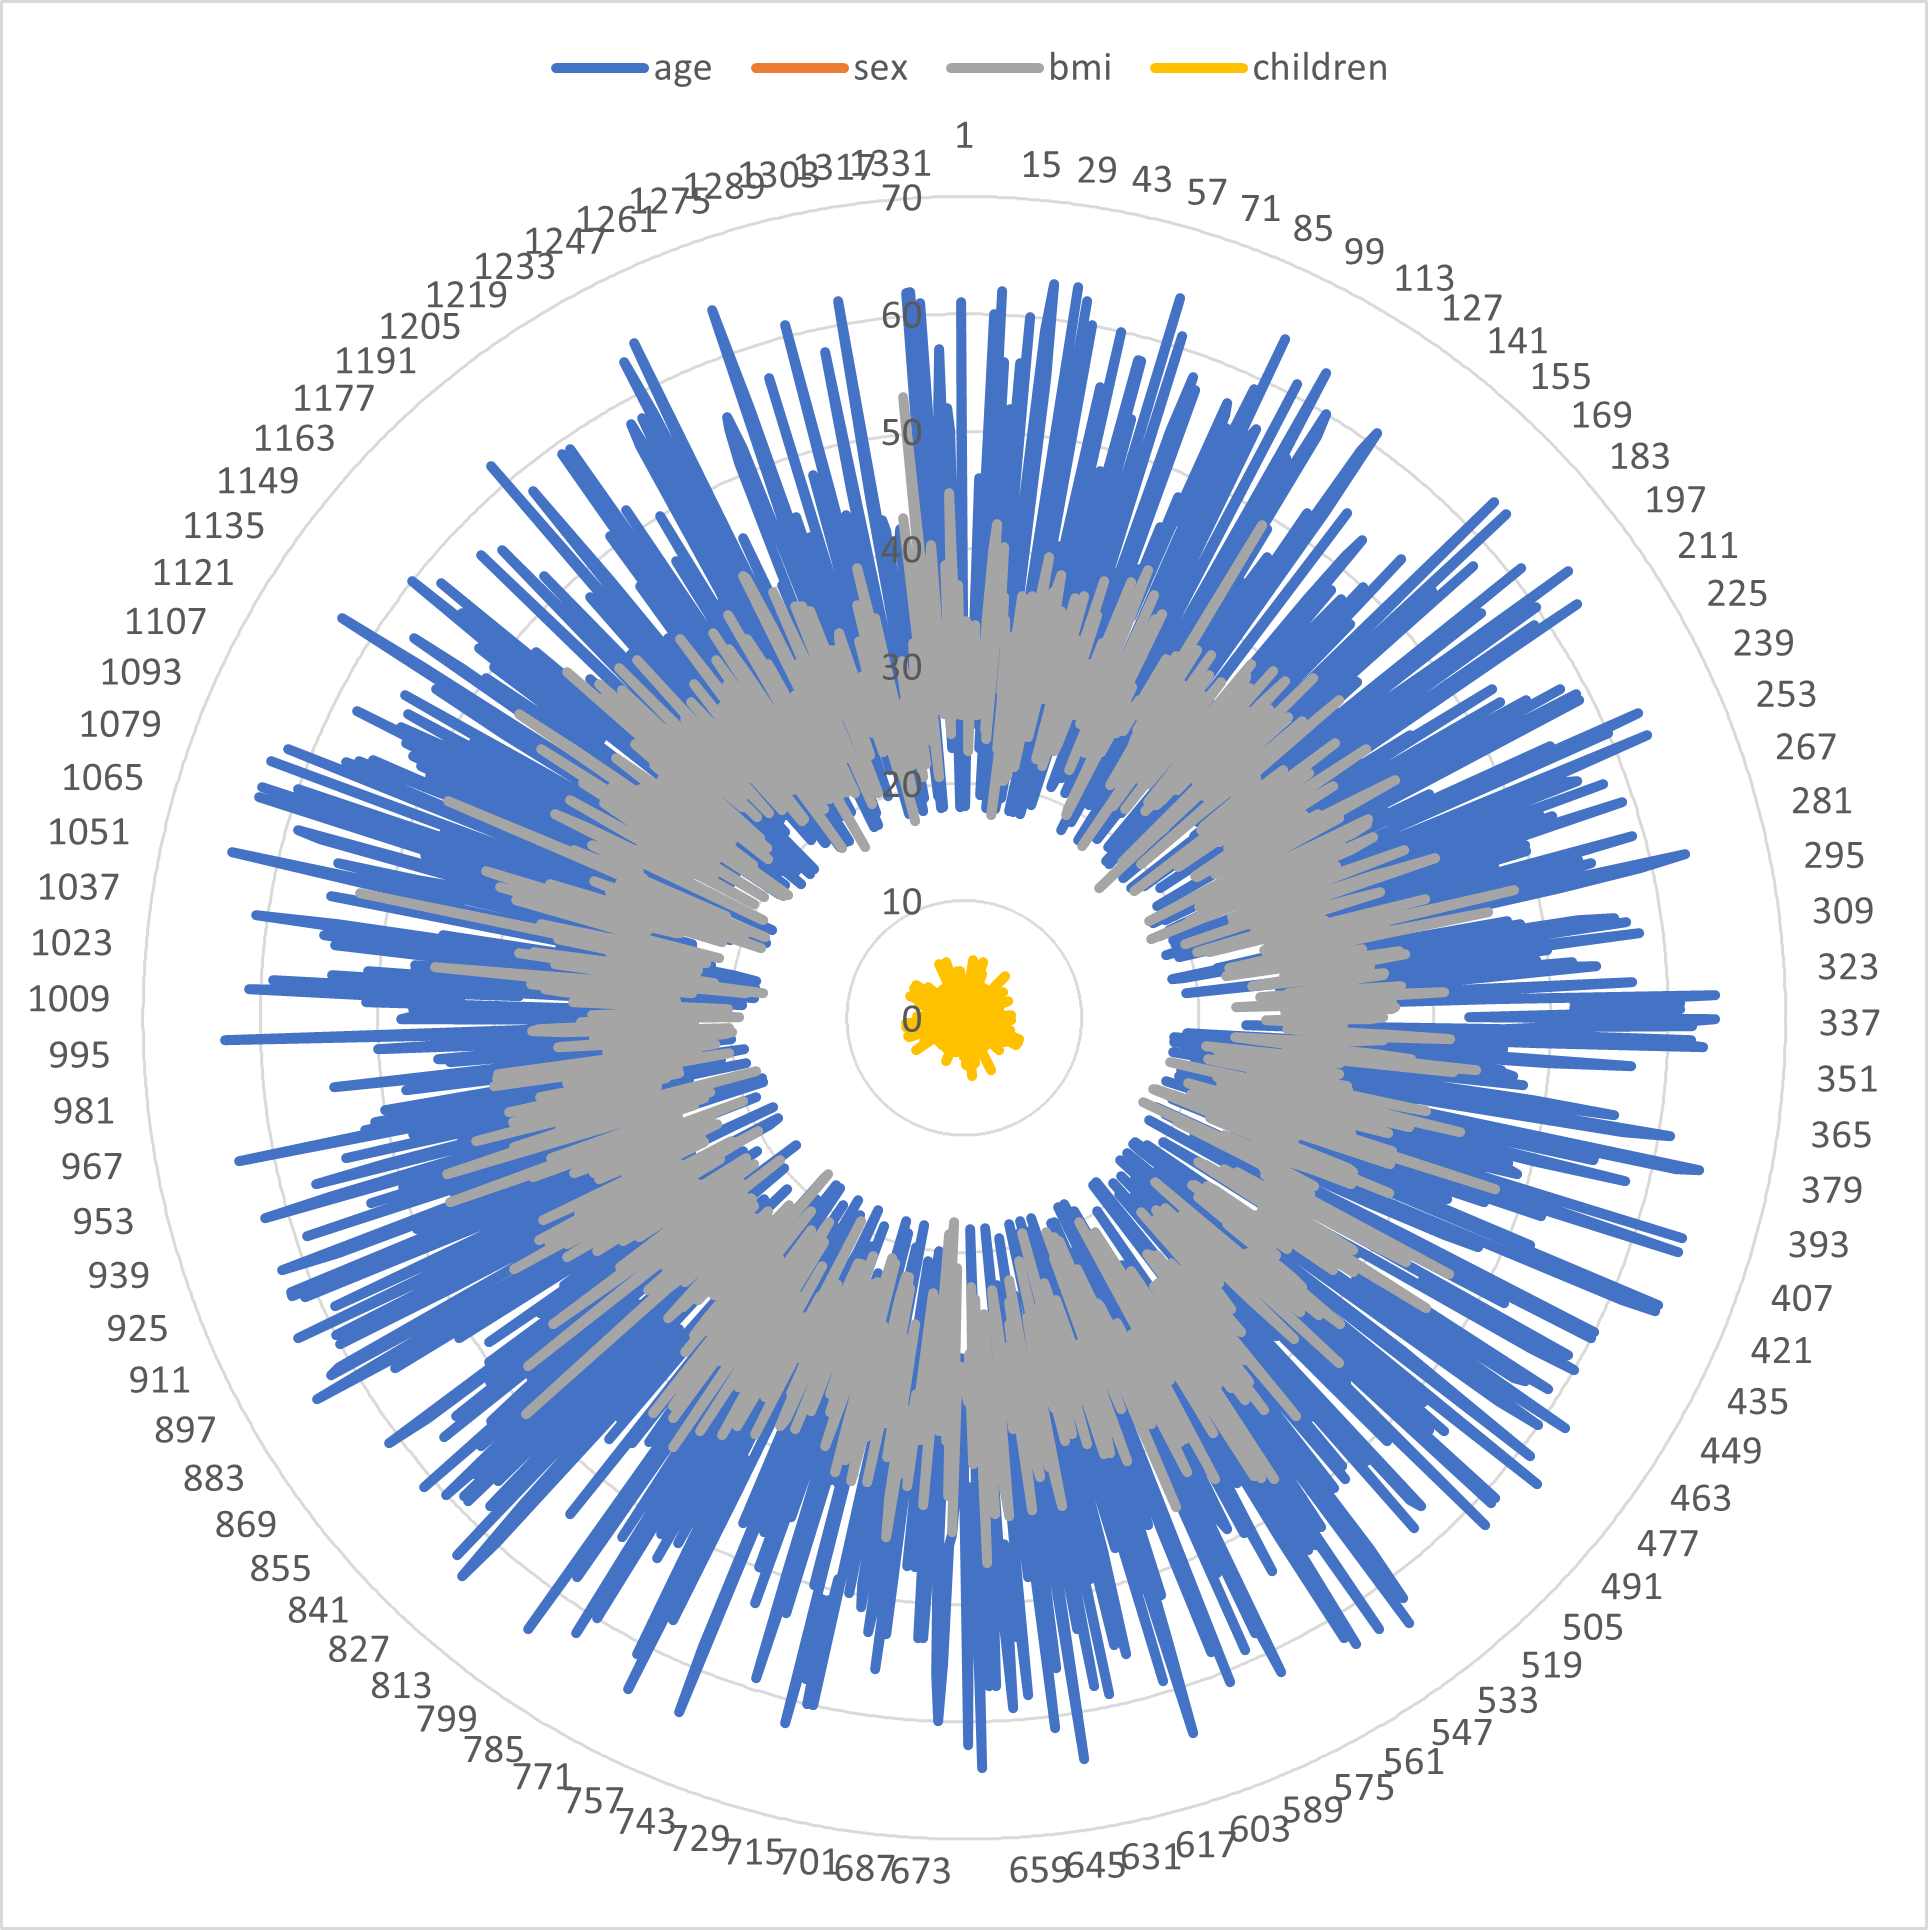
\includegraphics [width= 3.55 in]{10.png}
\caption{}
  \label{storage}
\end{figure}

\par Policy consulting market analysis reports and situational market analysis reports exposing operational circumstances are two categories of market analysis studies. Policy Consulting's market research report has a heavy focus on policy advice. A choice must be taken at any moment in order to build the appropriate market development policies as new circumstances, new objects, and new issues arise one after another throughout the process of economic and financial reform. The scenario and market analysis reports that show the operational conditions are used for a number of things. Understanding the market environment and the operational environment of banks may be utilized to carry out tasks, clarify the situation, and serve as a foundation for developing specific rules and regulations.

\par The market study report helps businesses understand market dynamics. The market research report is the company's window into the market's dynamics. If the business wishes to establish a strong footing in the market competition, increase its market share while preserving its current share, or create new ones, The characteristics of the market, including market supply and demand, current market trends, consumer demands, and product sales, must be completely understood in order to comprehend the market.

\par The market research study may serve as a foundation for businesses to assess their own level of competitiveness objectively and modify strategic plans for product development and manufacturing. If an organization wants to clarify its own position in the market competition, it must conduct market research and obtain reliable information from market research reports. The enterprise can ensure the right decision-making, find the right position, recognise its own shortcomings, maximise its strengths and avoid weaknesses, seek the best resource allocation, and pursue the goal of achieving high profits.

\par The market study report has evolved in recent years into a crucial foundation for business growth. It has a significant impact on how the business develops. The company's growth and the study of the market have been closely linked.


\bibliographystyle{IEEEtran}

%\bibliography{template} %-->reference list is on the template.bib file
\begin{thebibliography}{1.7} 
	\bibitem[1]{Septiawan1} \color{cyan}Kaggle. “Insurance Premium Data,” September 9, 2020. https://www.kaggle.com/datasets/simranjain17/insurance.\color{black}
        \bibitem[2]{Septiawan} \color{cyan} Kahneman, Daniel, and Amos Tversky. “Prospect Theory: An Analysis of Decision under Risk.” Econometrica 47, no. 2 (March 1979): 263. https://doi.org/10.2307/1914185.  \color{black}
        \bibitem[3]{Septiawa} \color{cyan} Cutler, David M., and Richard Zeckhauser. “Extending the Theory to Meet the Practice of Insurance.” Brookings-Wharton Papers on Financial Services 2004, no. 1 (2004): 1–53. https://doi.org/10.1353/pfs.2004.0002.  \color{black}
        \bibitem[4]{Septiaw} \color{cyan} Feldstein, Martin. “Rethinking Social Insurance.” American Economic Review 95, no. 1 (February 1, 2005): 1–24. https://doi.org/10.1257/00028280538285.  \color{black}
        \bibitem[5]{Septia} \color{cyan}Cochrane, John H. “A Simple Test of Consumption Insurance.” Journal of Political Economy 99, no. 5 (October 1991): 957–76. https://doi.org/10.1086/261785.  \color{black}
        \bibitem[6]{Septi} \color{cyan} Mills, Evan. “Insurance in a Climate of Change.” Science 309, no. 5737 (August 12, 2005): 1040–44. https://doi.org/10.1126/science.1112121. \color{black}
        \bibitem[7]{Sept} \color{cyan} Kataoka, Sheryl H., Lily Zhang, and Kenneth B. Wells. “Unmet Need for Mental Health Care Among U.S. Children: Variation by Ethnicity and Insurance Status.” American Journal of Psychiatry 159, no. 9 (September 2002): 1548–55. https://doi.org/10.1176/appi.ajp.159.9.1548. \color{black}
        \bibitem[8]{Sep} \color{cyan} Lewis, Frank D. “Dependents and the Demand for Life Insurance.” The American Economic Review 79, no. 3 (December 31, 1988): 452–67. https://econpapers.repec.org/RePEc:aea:aecrev:v:79:y:1989:i:3:p:452-67. \color{black}
        \bibitem[9]{Se} \color{cyan} Egenhofer, M.J. “Spatial SQL: A Query and Presentation Language.” IEEE Transactions on Knowledge and Data Engineering 6, no. 1 (1994): 86–95. https://doi.org/10.1109/69.273029. \color{black}
         \bibitem[10]{Septiawa1} \color{cyan}Kießling, Werner, and Gerhard Köstler. “Preference SQL — Design, Implementation, Experiences.” VLDB ’02: Proceedings of the 28th International Conference on Very Large Databases, 2002, 990–1001. https://doi.org/10.1016/b978-155860869-6/50098-6.\color{black}
        \bibitem[11]{Septawan1} \color{cyan} Spider: A Large-Scale Human-Labeled Dataset for Complex and Cross-Domain Semantic Parsing and Text-to-SQL Task \color{black}
         \bibitem[12]{Spiawan1} \color{cyan} Lewis, Frank D. “Dependents and the Demand for Life Insurance.” The American Economic Review 79, no. 3 (December 31, 1988): 452–67. https://econpapers.repec.org/RePEc:aea:aecrev:v:79:y:1989:i:3:p:452-67. \color{black}
        \bibitem[13]{Sepiawan1} \color{cyan}On optimizing an SQL-like nested query \color{black}
         \bibitem[14]{Septiawan1} \color{cyan}Kim, Won. “On Optimizing an SQL-like Nested Query.” ACM Transactions on Database Systems 7, no. 3 (September 1982): 443–69. https://doi.org/10.1145/319732.319745.\color{black}
        \bibitem[15]{Septiawan1} \color{cyan} Guo, Jiaqi, Zecheng Zhan, Yan Gao, Yan Xiao, Jian-Guang Lou, Ting Liu, and Dongmei Zhang. “Towards Complex Text-to-SQL in Cross-Domain Database with Intermediate Representation.” Proceedings of the 57th Annual Meeting of the Association for Computational Linguistics, 2019. https://doi.org/10.18653/v1/p19-1444.\color{black}
        \bibitem[16]{Setiawan1} \color{cyan}Wang, Bailin, Richard Shin, Xiaodong Liu, Oleksandr Polozov, and Matthew Richardson. “RAT-SQL: Relation-Aware Schema Encoding and Linking for Text-to-SQL Parsers.” Proceedings of the 58th Annual Meeting of the Association for Computational Linguistics, 2020. https://doi.org/10.18653/v1/2020.acl-main.677.\color{black}
        \bibitem[17]{Sepiawan1} \color{cyan}On optimizing an SQL-like nested query \color{black}
         \bibitem[18]{Septwan1} \color{cyan}Hellerstein, Joe, Christopher Ré, Florian Schoppmann, Daisy Zhe Wang, Eugene Fratkin, Aleksander Gorajek, Kee Siong Ng, et al. “The MADlib Analytics Library or MAD Skills, the SQL.” Cornell University - ArXiv, August 19, 2012. https://doi.org/10.48550/arxiv.1208.4165.\color{black}
        \bibitem[19]{Septan1} \color{cyan}Anisimova, Maria, and Olivier Gascuel. “Approximate Likelihood-Ratio Test for Branches: A Fast, Accurate, and Powerful Alternative.” Edited by Jack Sullivan. Systematic Biology 55, no. 4 (August 1, 2006): 539–52. https://doi.org/10.1080/10635150600755453.\color{black}
        \bibitem[20]{Septibawan1} \color{cyan}Kießling, Werner, and Gerhard Köstler. “Preference SQL — Design, Implementation, Experiences.” VLDB ’02: Proceedings of the 28th International Conference on Very Large Databases, 2002, 990–1001. https://doi.org/10.1016/b978-155860869-6/50098-6.\color{black}
         \bibitem[21]{Sebptiawan1} \color{cyan} Lewis, Frank D. “Dependents and the Demand for Life Insurance.” The American Economic Review 79, no. 3 (December 31, 1988): 452–67. https://econpapers.repec.org/RePEc:aea:aecrev:v:79:y:1989:i:3:p:4232-67. \color{black}
         \bibitem[22]{Septiawan1} \color{cyan} Mills, Evan. “Insurance in a Climate of Change.” Science 309, no. 5737 (August 12, 2005): 1040–44. https://doi.org/10.1246/science.12465345. \color{black}
         \bibitem[23]{Septikawan1} \color{cyan} Chandra, Yanto, and Liang Shang. “An RQDA-Based Constructivist Methodology for Qualitative Research.” Qualitative Market Research: An International Journal 20, no. 1 (January 9, 2017): 90–112. https://doi.org/10.1108/qmr-02-2016-0014. \color{black}
         \bibitem[24]{Septimawan1} \color{cyan}McMurdie, Paul J., and Susan Holmes. “Phyloseq: An R Package for Reproducible Interactive Analysis and Graphics of Microbiome Census Data.” Edited by Michael Watson. PLoS ONE 8, no. 4 (April 22, 2013): e61217. https://doi.org/10.1371/journal.pone.0061217. \color{black}
          \bibitem[25]{Septidhawan1} \color{cyan}Hussain, Mohammed, G. Yedukondalu, Y. Kamala Raju, and V. Kamakshi Prasad. “Comparison of Methods of Prediction of Compressive Strength of Concrete Using Multiple Linear Regression in Microsoft Excel and Artificial Neural Networks in RStudio.” SEVENTH INTERNATIONAL SYMPOSIUM ON NEGATIVE IONS, BEAMS AND SOURCES (NIBS 2020), 2021. https://doi.org/10.1063/5.0058070. \color{black}
         \bibitem[26]{Septieanjn1} \color{cyan}Shapiro, Heather B., Clara H. Lee, Noelle E. Wyman Roth, Kun Li, Mine Çetinkaya-Rundel, and Dorian A. Canelas. “Understanding the Massive Open Online Course (MOOC) Student Experience: An Examination of Attitudes, Motivations, and Barriers.” Computers &Amp; Education 110 (July 2017): 35–50. https://doi.org/10.1016/j.compedu.2017.03.003. \color{black}
          \bibitem[27]{Septihhan1} \color{cyan}Satorra, Albert, and Willem E. Saris. “Power of the Likelihood Ratio Test in Covariance Structure Analysis.” Psychometrika 50, no. 1 (March 1985): 83–90. https://doi.org/10.1007/bf02294150.\color{black}
        
         

 
	
 

 
\end{thebibliography}



\end{document}

%\begin{figure}[!t]
%\centering
%\includegraphics[width=2.5in]{myfigure}
% where an .eps filename suffix will be assumed under latex, 
%\caption{Simulation results for the network.}
%\label{fig_sim}
%\end{figure}